%----------------------------------------------------------------------------------------
%    PACKAGES AND THEMES
%----------------------------------------------------------------------------------------

\documentclass[aspectratio=169,xcolor=dvipsnames]{beamer}
\usepackage{caption}
\usepackage{biblatex}
\addbibresource{references.bib} 
\usepackage{hyperref}
\usepackage{graphicx} % Allows including images
\usepackage{booktabs} % Allows the use of \toprule, \midrule and \bottomrule in tables
\setbeamertemplate{footline}[frame number] % Adds slide numbers to the footer
\usepackage{amsmath} % Allows the use of mathematical symbols and environments
\usepackage{amsthm} % Allows the use of theorem environments
\usepackage{amssymb} % Allows the use of additional mathematical symbols
\usepackage{multicol} % Allows the use of multiple columns in a slide
\usepackage{algorithm} % For algorithm environment
\usepackage{algpseudocode} % For algorithmic environment

\usepackage[progressbar=yes,framecount=fancy]{BeamerTheme}
%----------------------------------------------------------------------------------------
%    TITLE PAGE
%----------------------------------------------------------------------------------------

\title{On the Exact Separation of \\ Mixed Integer Knapsack Cuts}

\author{
Guillem Audebert, 
Léonard Bultinck,
Tudor Cardas,
Yağmur Ergin}
\date{\today} % Date, can be changed to a custom date
%----------------------------------------------------------------------------------------
%    PRESENTATION SLIDES
%----------------------------------------------------------------------------------------

\begin{document}

\begin{frame}{Overview}
    % Automatically generates a table of contents based on \section{} and \subsection{}
    \tableofcontents
\end{frame}

%------------------------------------------------
\section{Introduction}
%------------------------------------------------

\begin{frame}{Introduction}
    \vspace{-0.2cm}
    \begin{columns}[T]
        \begin{column}{0.48\textwidth}
            \textbf{Mixed Integer Knapsack Set :} \\
            \small
            Consider a positive integer $n$, $b \in \mathbb{Q}$, $a \in \mathbb{Q}^n$, $l \in \{\mathbb{Q} \cup \{-\infty\}\}^n$, $u \in \{\mathbb{Q} \cup \{+\infty\}\}^n$ and $I \subseteq N := \{1, \ldots, n\}$
            \[
            K = \{x \in \mathbb{R}^n : ax \leq b, l \leq x \leq u, x_i \in \mathbb{Z}, \forall i \in I \}
            \]
            Given a point $x^* \in \mathbb{Q}^n$
            \begin{itemize}
                \item Identify an inequality ($\pi x \leq \pi_0$) valid for conv$(K)$ and violated by $x^*$.
                \item Prove that no such inequality exists.
            \end{itemize}
        \end{column}
        \hspace{0.5cm}
        \begin{column}{0.48\textwidth}
            \textbf{Mixed Integer Set : } \\
            \vspace{-0.4cm}
            \small
            \[
            P = \{x \in \mathbb{R}^n : Dx \leq d, l \leq x \leq u, x_i \in \mathbb{Z}, \forall i \in I \}
            \]
            $D$ is an $m \times n$ matrix, and $d \in \mathbb{Q}^n$\\
            \vspace{0.3cm}
            If $(a, b)$ can be obtained as a non-negative linear combination of rows from $(D, d)$, then $P \subseteq K$ 
            and we say that $K$ is an implied knapsack set of $P$. 
        \end{column}
    \end{columns}
\end{frame}
%------------------------------------------------
\section{Identifying a Violated Knapsack Cut}
%------------------------------------------------
\begin{frame}{Is $x^* \in \text{conv}(K)$?}
    \vspace{-0.4cm}
    \textbf{Suggestion:} Solve the following linear program to solve the separation problem:
    \vspace{-0.4cm}
    \begin{align*}
    LP_1 : \min \quad & \sum_{i=1}^{n} (u_i + v_i) \\
    \text{s.t.} \quad & \pi x^k - \pi_0 \leq 0 & \forall k = 1, \ldots, q & \quad \text{(C1)} \\
    & \pi r^k \leq 0 & \forall k = 1, \ldots, t & \quad \text{(C2)} \\
    & \pi x^* - \pi_0 = 1 & & \quad \text{(C3)} \\
    & \pi + u - v = 0 & & \quad \text{(C4)} \\
    & u \geq 0, \; v \geq 0 & &
    \end{align*}
    \vspace{-0.1cm}
    If $LP_1$ is infeasible, then $x^* \in \text{conv}(K)$.\\ 
    Otherwise, the optimal solution $(u, v, \pi, \pi_0)$ gives a valid knapsack cut $\pi x \leq \pi_0$.
\end{frame}

\begin{frame}{Algorithm}
    \begin{algorithm}[H]
    \caption{knapsack\_separator($K$, $x^*$)}
    \small
    \textbf{Input:} A MIK set $K$, and a vector $x^*$.\\
    \textbf{Output:} If $x^* \in \text{conv}(K)$ : TRUE; Else : FALSE and a cut separating $x^*$ from $\text{conv}(K)$\\
    \vspace{-0.4cm}
    \begin{algorithmic}[1]
    \State Simplify the problem by fixing variables which are at their bounds, and reduce to a smaller dimensional knapsack separation problem;
    \State Formulate problem $LP_1$ in the reduced variable space without $(C1) - (C2)$;
    \State Apply P1-P2 to simplify $LP_1$;
    \State Solve $LP_1$ using the dynamic row generation algorithm;
    \State If solving $LP_1$ reveals that $x^* \in \text{conv}(K)$ : STOP and return TRUE;
    \State Let $(\hat{\pi}, \hat{\pi}_0)$ represent the optimal solution to $LP_1$;
    \State Lift cut $\hat{\pi} x \leq \hat{\pi}_0$ to obtain a cut $\pi x \leq \pi_0$ which is valid for $K$;
    \State STOP and return the cut $(\pi, \pi_0)$;
    \end{algorithmic}
    \end{algorithm}
\end{frame}

%------------------------------------------------
\section{Solving the Mixed Integer Knapsack Problem}
%------------------------------------------------


%%%%%%%%%%%%%%% Guillem

\subsection{Reducing the problem}
\begin{frame}{Is $x^* \in \text{conv}(K)$ ?}
	
	\begin{block}{$LP_1$ and knapsack cut}
		\begin{itemize}
			\item If not, exhibit a cut $\pi x \leq \pi_0$ 
			\item Constraint $ \pi x^k - \pi_0 \leq 0 \; , \forall x^k$ being an extreme point $\text{conv}(K)$.
			\item $\implies $ exponential number of rows.
			\item Too many $\pi$ variables.
		\end{itemize}
	\end{block}
	
	\begin{center}
		$\Rightarrow$ \textbf{Simplify $LP_1$ before solving it}
	\end{center}
	
    
\end{frame}


\begin{frame}{Eliminate variables \& Tighten $LP_1$}

	\begin{block}{Proposition 1 : Using property of valid cuts}
		\begin{itemize}
			\item Sign coherence: $a_i > 0 \Rightarrow \pi_i \geq 0$ \quad ; \quad $a_i < 0 \Rightarrow \pi_i \leq 0$
			\item Unbounded continuous variables $\Rightarrow$ \textbf{eliminate} or replace by $\alpha \cdot a_i$
		\end{itemize}
	\end{block}


\end{frame}



\begin{frame}{Eliminate variables \& Tighten $LP_1$}
	\begin{block}{ Proposition 2 : Using position of $x^*$}
		
			Variables at bounds in "right direction" $\Rightarrow$ set $\pi_i = 0$
			\begin{itemize}
				\item $a_i > 0$ and $x^*_i = l_i$ $\Rightarrow$ $\pi_i = 0$
				\item $a_i < 0$ and $x^*_i = u_i$ $\Rightarrow$ $\pi_i = 0$
			\end{itemize}

	\end{block}
\end{frame}



\begin{frame}{Reducing Dimension}
	\begin{block}{Fixing \& Lifting}
		\begin{itemize}
			\item Fix variable that are already at bounds. (Fixing)
			\item  Solve on Smaller Space $K(L,U)$
			\item Reintroduces  fixed variables (Lifting)
		\end{itemize}
	\end{block}
	
	\vspace{0.3cm}
	\begin{alertblock}{Combined effect}
		Transform unsolvable $LP_1$ into computable problem
	\end{alertblock}
\end{frame}


%%%%%%%%%%%%%%%%%%%%%%%%%%%%%%

\subsection{B}
\begin{frame}{1}
    \begin{itemize}
        \item a
        \item b
    \end{itemize}
\end{frame}
%------------------------------------------------
%Leonard
\section{Computational Results}

\begin{frame}{Experimental Setup}
The computational results are based on \textbf{67 instances} of the knapsack problem.

\begin{itemize}
    \item These instances are selected from an initial set of approximately \textbf{130,000 instances}.
    \item Most of the instances are similar; therefore, only the \textbf{latest (supposedly hardest)} instance of each group is kept.
    \item The \textbf{easiest instances} (solved in less than 1 second) are removed.
\end{itemize}

\medskip
Removing very easy instances reduces sensitivity to small time variations and avoids bias in performance comparisons.
\end{frame}

\begin{frame}{Limitations of the Instance Selection}
Despite the above filtering, using only \textbf{67 instances} may appear insufficient for a robust comparison.

\begin{itemize}
    \item The original 130,000 instances are drawn from \textbf{MIPLIB}.
    \item The selection process is not fully described, making the results \textbf{non-reproducible}.
    \item Fortunately, the authors make the full set of instances \textbf{available upon request}.
\end{itemize}
\end{frame}

\begin{frame}{Analysis of the Performance Graph}
The performance graph is difficult to read but provides valuable information.

\begin{itemize}
    \item It shows which solver performs best on a given \textbf{percentage of instances}.
    \item This provides a notion of \textbf{average dominance or “betterness”}.
    \item The curve also indicates the percentage of instances for which a solver is more than $x$ times slower than another.
\end{itemize}

Overall, it is an effective way to compare solvers across multiple instances.
\end{frame}

\begin{frame}{Discussion and Limitations}
While this approach is useful, it has some limitations.

\begin{itemize}
    \item As more solvers are added, the graph becomes harder to interpret.
    \item The use of an \textbf{OR condition on the y-axis} leads to information loss.
\end{itemize}

Thus, although informative, the visualization does not scale well with an increasing number of solvers.
\end{frame}

\begin{frame}{Results}
\begin{figure}
    \centering
    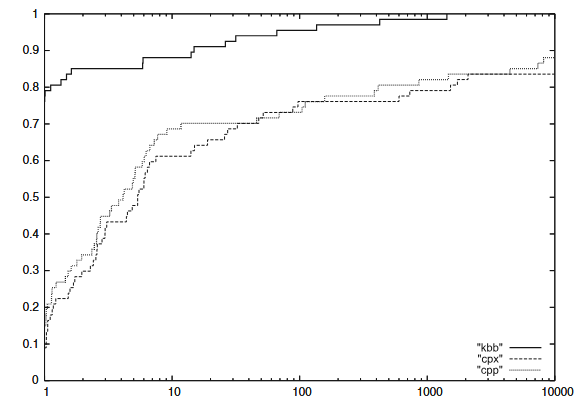
\includegraphics[width=0.8\textwidth]{figure1}
    \caption{Performance comparison of solvers on knapsack instances}
\end{figure}
\end{frame}

\begin{frame}{Comparative Analysis}
The comparison highlights the strong performance of the proposed algorithm, \textbf{KBB}.

\begin{itemize}
    \item KBB improves rapidly along the performance graph $\implies$ no instances inherently hard for the algorithm
    \item It is \textbf{never more than 1000 times slower} than any competing solver on any instance.
    \item KBB performs best on approximately \textbf{77\% of the instances}.
    \item There are \textbf{two instances} that could not be solved by either \textbf{CPX} or \textbf{CPP}, while \textbf{KBB} successfully solved them.
\end{itemize}

Overall, these results indicate both robustness and competitive efficiency of KBB.
\end{frame}

\begin{frame}{Enhancement results}
\begin{figure}
    \centering
    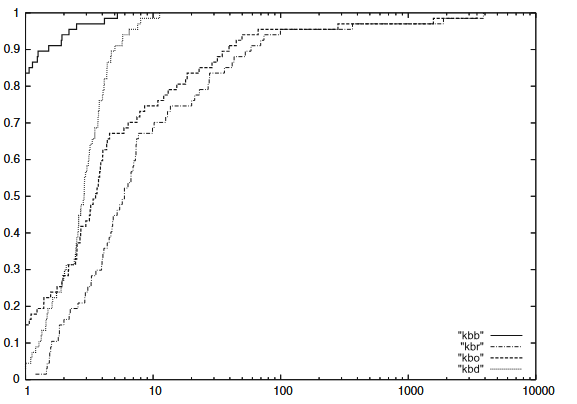
\includegraphics[width=0.8\textwidth]{figure2}
    \caption{Performance comparison of enhancement induced by domination branching or reduced-cost bound improvement}
\end{figure}
\end{frame}

\begin{frame}{Enhancement Analysis}


\begin{itemize}
    \item When applied independently, the enhancements do not reduce the search space and may even slow down the algorithm.
    \item When combined, however, they lead to a \textbf{significant performance improvement}.
    \item These two features naturally complement each other.
    \item Updating bounds enables additional domination conditions to be applied.
    \item This interaction results in \textbf{further pruning of the search tree}.
\end{itemize}
\end{frame}
%------------------------------------------------
\section{Conclusion}
%------------------------------------------------

\begin{frame}{Conclusion}
    blablabla
\end{frame}

%------------------------------------------------
\begin{frame}{References}
%------------------------------------------------

    \tiny
    \begin{multicols}{2} 
        \printbibliography[heading=none]
    \end{multicols}
\end{frame}

%------------------------------------------------
\begin{frame}
    \Huge{\centerline{\textbf{Questions?}}}
\end{frame}

%----------------------------------------------------------------------------------------

\end{document}
